% AKULIN R2 CP07 -- published spectroscopy fig. 17.6 (qualitative trace).
% Pixel-landmark reconstruction from the printed original, NOT measured raw data.
% One broad trace (a); one structured SF6 printed contour (b), with its narrow
% and shoulder extrema separately retained (rather than a fitted smooth spectrum).
\documentclass[border=6pt]{standalone}
\usepackage{fontspec,unicode-math}
\setmainfont{Noto Serif}
\setmathfont{STIXTwoMath-Regular.otf}
\usepackage{tikz}
\usetikzlibrary{arrows.meta}
\tikzset{
 curve/.style={draw=black,line width=.88pt,line cap=round,line join=round},
 axis/.style={draw=black,line width=.62pt,-{Latex[length=2mm,width=1mm]}},
 tick/.style={draw=black,line width=.45pt},
 lab/.style={font=\fontsize{10.5}{13}\selectfont,inner sep=.5pt},
 panel/.style={font=\fontsize{13}{15}\selectfont\itshape,inner sep=.7pt}}
\begin{document}
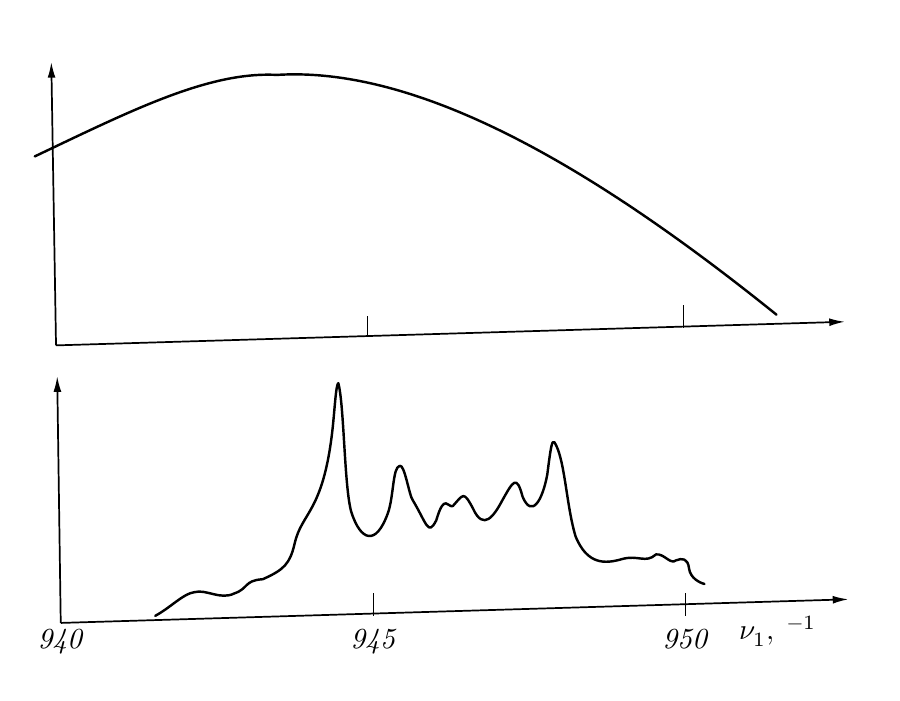
\begin{tikzpicture}[x=.015cm,y=-.015cm]
\path[use as bounding box] (0,0) rectangle (715,546);
% The author does not supply y-axis calibration for these two panels.
% Upper broad absorption profile retains its asymmetric maximum and right tail.
\draw[curve] (6,109)
 .. controls (90,69) and (154,37) .. (211,40)
 .. controls (337,32) and (490,127) .. (634,243);
\draw[axis] (24,269)--(20,29);
\draw[axis] (24,269)--(692,249);
\draw[tick] (288,262)--(288,244);
\draw[tick] (555,254)--(555,235);
\node[panel] at (584,70) {а};
% Lower trace: print-derived local features. Deliberately non-Gaussian and
% non-periodic small ripples; no line interpolation pretending to be data.
\draw[curve] (108,498)
 .. controls (121,491) and (132,479) .. (141,478)
 .. controls (151,475) and (163,485) .. (175,479)
 .. controls (187,475) and (183,468) .. (199,467)
 .. controls (217,459) and (222,454) .. (226,437)
 .. controls (232,410) and (250,411) .. (258,341)
 .. controls (260,323) and (261,302) .. (263,301)
 .. controls (268,319) and (268,389) .. (274,410)
 .. controls (282,435) and (295,439) .. (305,411)
 .. controls (310,397) and (309,372) .. (315,371)
 .. controls (319,369) and (323,396) .. (326,400)
 .. controls (338,420) and (339,431) .. (346,417)
 .. controls (353,393) and (356,407) .. (360,405)
 .. controls (369,395) and (369,392) .. (377,407)
 .. controls (386,427) and (395,413) .. (402,400)
 .. controls (411,384) and (414,378) .. (419,397)
 .. controls (427,416) and (436,400) .. (440,378)
 .. controls (443,354) and (444,349) .. (446,351)
 .. controls (455,365) and (456,405) .. (464,431)
 .. controls (474,455) and (489,454) .. (503,450)
 .. controls (517,446) and (523,454) .. (532,446)
 .. controls (539,445) and (544,455) .. (549,451)
 .. controls (554,449) and (559,449) .. (560,458)
 .. controls (561,466) and (569,470) .. (573,471);
\draw[axis] (28,504)--(25,295);
\draw[axis] (28,504)--(695,484);
\foreach \x/\value in {28/940,293/945,557/950}{
  \draw[tick] (\x,498)--(\x,479);
  \node[lab,anchor=north] at (\x,508) {$\mathit{\value}$};
}
\node[lab,anchor=west] at (601,511) {$\nu_1,\;\mathrm{см}^{-1}$};
\node[panel] at (595,295) {б};
\end{tikzpicture}
\end{document}
